%!TEX root = ../../Master.tex
\subsection{CrustCrawler}

AX-12A Smart Robotic Arm er den robot, som universitetet har stillet til rådighed til dette projekt. Robotten er designet som en arm med en baserotation, en skulderrotation, en underarmsrotation samt en håndledsrotation. Desuden er der monteret en gripper for enden af armen, som gør det muligt at samle ting op. Et billede af robotten ses på \autoref{fig:crustcrawler}. Som det ses på billedet kan et led mellem baserotationen og skulderrotationen sættes fast i en anden position end lige op. \\

\fixme{Ændre 'Figure' til 'Figur'}

\begin{figure}[h]
\centering
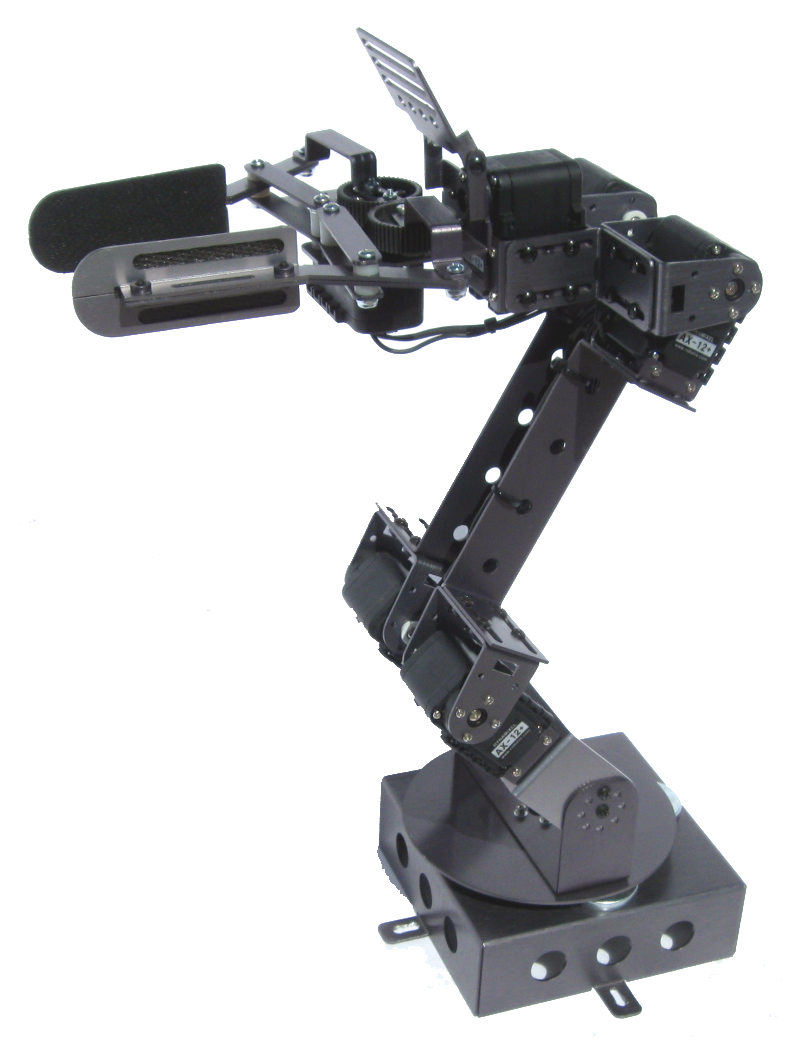
\includegraphics[scale=0.45]{images/crustCrawler}
\caption{AX-12A Smart Robotic Arm fra CrustCrawler Robotics}
\label{fig:crustcrawler}
\end{figure}

Robotten er 56,51 cm lang fra base til gripper og vejer 1 kg. Robotten har 4 frihedsgrader, hvilket betyder at den ikke er i stand til at nå alle steder, som ellers er inden for rækkevide. Hvis dette skulle have været muligt, skulle robotten have været i besidelse af 6 frihedsgrader. Hvis det er nødvendigt at nå et punkt, som robotten ikke kan, kan det hjælpe at ændre leddet mellem baserotationen og skulderrotationen til en anden fast position. Robottens løftekapacitet kan nå op på 1,36 kg.
